\documentclass{report}

\usepackage[english]{babel}
\usepackage[utf8]{inputenc}
% for using coloring, used in code blocks and linking
\usepackage{color}
% for hrefs and urls
\usepackage[hidelinks]{hyperref}
\hypersetup{
	hidelinks = true,
	colorlinks = true,
	citecolor = darkgray,
	linkcolor = black,
	urlcolor = blue
}
% for code blocks
\usepackage{listings}
% for using maths or symbols
\usepackage{amssymb}
%adding bibliography to TOC
\usepackage[nottoc]{tocbibind}
% for images
\usepackage{graphicx}
\usepackage{wrapfig}
% image path
\graphicspath{ {figures/} }
% using images inline with text
\usepackage{wrapfig}
% some latex-fu for html-xml-css-js stuff
\definecolor{darkblue}{rgb}{0.0,0.0,0.6}
\definecolor{cyan}{rgb}{0.0,0.6,0.6}
\definecolor{lightgray}{rgb}{0.95, 0.95, 0.95}
\definecolor{darkgray}{rgb}{0.4, 0.4, 0.4}
\definecolor{editorGray}{rgb}{0.95, 0.95, 0.95}
\definecolor{editorOcher}{rgb}{1, 0.5, 0} % #FF7F00 -> rgb(239, 169, 0)
\definecolor{editorGreen}{rgb}{0, 0.5, 0} % #007C00 -> rgb(0, 124, 0)
\definecolor{orange}{rgb}{1,0.45,0.13}      
\definecolor{olive}{rgb}{0.17,0.59,0.20}
\definecolor{brown}{rgb}{0.69,0.31,0.31}
\definecolor{purple}{rgb}{0.38,0.18,0.81}
\definecolor{lightblue}{rgb}{0.1,0.57,0.7}
\definecolor{lightred}{rgb}{1,0.4,0.5}

\lstset{
  basicstyle=\footnotesize\ttfamily,
  columns=fullflexible,
  showstringspaces=false,
  commentstyle=\color{darkgray}\upshape
}

\lstdefinestyle{code}{
  % line-numbers
  xleftmargin={0.75cm},
  numbers=left,
  stepnumber=1,
  firstnumber=1,
  numberfirstline=true,
}

\lstdefinelanguage{XML}{
  morestring=[b]",
  morestring=[s]{>}{<},
  morecomment=[s]{<?}{?>},
  stringstyle=\color{black},
  identifierstyle=\color{darkblue},
  keywordstyle=\color{cyan},
  morekeywords={xmlns,version,type}% list your attributes here
}

\lstdefinestyle{xml}{
  % line-numbers
  xleftmargin={0.75cm},
  numbers=left,
  stepnumber=1,
  firstnumber=1,
  numberfirstline=true,
  language=XML, 
  alsodigit={.:;},  
  tabsize=2,
  showtabs=false,
  showspaces=false,
  showstringspaces=false,
  extendedchars=true,
  breaklines=true,
}

% CSS
\lstdefinelanguage{CSS}{
  keywords={color,background-image:,margin,padding,font,weight,display,position,top,left,right,bottom,list,style,border,size,white,space,min,width, transition:, transform:, transition-property, transition-duration, transition-timing-function}, 
  sensitive=true,
  morecomment=[l]{//},
  morecomment=[s]{/*}{*/},
  morestring=[b]',
  morestring=[b]",
  alsoletter={:},
  alsodigit={-}
}

% JavaScript
\lstdefinelanguage{JavaScript}{
  morekeywords={typeof, new, true, false, catch, function, return, null, catch, switch, var, if, in, while, do, else, case, break},
  morecomment=[s]{/*}{*/},
  morecomment=[l]//,
  morestring=[b]",
  morestring=[b]'
}

\lstdefinelanguage{HTML5}{
  language=html,
  sensitive=true,   
  alsoletter={<>=-},    
  morecomment=[s]{<!-}{-->},
  tag=[s],
  otherkeywords={
  % General
  >,
  % Standard tags
    <!DOCTYPE,
  </html, <html, <head, <title, </title, <style, </style, <link, </head, <meta, />,
    % body
    </body, <body,
    % Divs
    </div, <div, </div>, 
    % Paragraphs
    </p, <p, </p>,
    % scripts
    </script, <script,
  % More tags...
  <canvas, /canvas>, <svg, <rect, <animateTransform, </rect>, </svg>, <video, <source, <iframe, </iframe>, </video>, <image, </image>, <header, </header, <article, </article
  },
  ndkeywords={
  % General
  =,
  % HTML attributes
  charset=, src=, id=, width=, height=, style=, type=, rel=, href=,
  % SVG attributes
  fill=, attributeName=, begin=, dur=, from=, to=, poster=, controls=, x=, y=, repeatCount=, xlink:href=,
  % properties
  margin:, padding:, background-image:, border:, top:, left:, position:, width:, height:, margin-top:, margin-bottom:, font-size:, line-height:,
    % CSS3 properties
  transform:, -moz-transform:, -webkit-transform:,
  animation:, -webkit-animation:,
  transition:,  transition-duration:, transition-property:, transition-timing-function:,
  }
}

\lstdefinestyle{htmlcssjs} {%
  % General design
%  backgroundcolor=\color{editorGray},
  basicstyle={\footnotesize\ttfamily},   
  %frame=b,
  % line-numbers
  xleftmargin={0.75cm},
  numbers=left,
  stepnumber=1,
  firstnumber=1,
  numberfirstline=true, 
  % Code design
  identifierstyle=\color{black},
  keywordstyle=\color{blue}\bfseries,
  ndkeywordstyle=\color{editorGreen}\bfseries,
  stringstyle=\color{editorOcher}\ttfamily,
  commentstyle=\color{brown}\ttfamily,
  % Code
  language=HTML5,
  alsolanguage=JavaScript,
  alsodigit={.:;},  
  tabsize=2,
  showtabs=false,
  showspaces=false,
  showstringspaces=false,
  extendedchars=true,
  breaklines=true,
  % German umlauts
  literate=%
  {Ö}{{\"O}}1
  {Ä}{{\"A}}1
  {Ü}{{\"U}}1
  {ß}{{\ss}}1
  {ü}{{\"u}}1
  {ä}{{\"a}}1
  {ö}{{\"o}}1
}

\title{ES lab-6, \LaTeX\ group exercise G2}
\author{Curran, T.; Maarse, M.; van Prooijen, J.}

\begin{document}
	\maketitle{}
	\tableofcontents
	\chapter{Introduction}
	This document is the \LaTeX\ representation of the first group exercises of group G2, during the SNE course of 2015-2016. During the making of this document a steep learning curve was achieved. Thanks to the assistents and \href{https://en.wikibooks.org/wiki/LaTeX}{wikibooks.org}\cite{wikibooks_latex_home} we've made it to a good end.
	\chapter{The Quest For XQuery}
Group G2, seats 6-11, subject XQuery.\\
For the groups result look: \href{https://www.os3.nl/2015-2016/students/jeroen_van_prooijen/es/week36/g2_exercise_xquery}{here}.\\
For the page describing this document look: \href{https://www.os3.nl/2015-2016/students/jeroen_van_prooijen/es/week36#group_assignmentxquery}{here}.\\

This \LaTeX\ chapter is made by Jeroen van Prooijen. Making this \LaTeX\ based representation of our wiki I've used overleaf for the color encoding of html and xml \cite{overleaf}.
To show that also labeling works, here a label of the image I've used. Figure: \ref{fig:w3schools_logo} shows the w3schools logo.

\section{Notes}
\begin{itemize}
\item XQuery is SQL for XML (\url{w3schools.com})
\end{itemize}

My task was to find information about the history and versions available on XQuery.

\begin{itemize}
\item XQuery 1.0 \hfill \\
$\rightarrow$ \href{http://www.w3.org/TR/xquery/}{Recommendation} presented in December 2010.
\item XQuery 3.0 \hfill \\
$\rightarrow$ \href{http://www.w3.org/TR/xquery-30/}{Recommendation} presented in April 2014.
\item XQuery 3.1 \hfill \\
$\rightarrow$ \href{http://www.w3.org/TR/xquery-3/}{Candidate recommendation} in December 2014 \\ 
$\rightarrow$ last \href{http://www.w3.org/TR/xquery-31-requirements/}{Group Note} is from August
\end{itemize}

\newpage

\section{Online interpreter for Xquery}

\begin{figure}[h]
\centering

\includegraphics[scale=1]{w3schools.jpg}
\caption{w3schools logo\cite{w3schools}}
\label{fig:w3schools_logo}
\end{figure}

I've used the examples on:
\begin{itemize}
\item \url{http://www.w3schools.com/xsl/xquery_example.asp}
\item \url{http://www.w3schools.com/xsl/xquery_flwor.asp}
\end{itemize}

And used the books.xml file, below: 

\begin{lstlisting}[style=xml, frame=single, caption={books.xml}]
<bookstore id="store">  
  <book category="COOKING">
    <title lang="en">Everyday Italian</title>
    <author>Giada De Laurentiis</author>
    <year>2005</year>
    <price>30.00</price>
  </book>
    <book category="CHILDREN">
    <title lang="en">Harry Potter</title>
    <author>J K. Rowling</author>
    <year>2005</year>
    <price>29.99</price>
  </book>
  <book category="WEB">
    <title lang="en">XQuery Kick Start</title>
    <author>James McGovern</author>
    <author>Per Bothner</author>
    <author>Kurt Cagle</author>
    <author>James Linn</author>
    <author>Vaidyanathan Nagarajan</author>
    <year>2003</year>
    <price>49.99</price>
  </book>
  <book category="WEB">
    <title lang="en">Learning XML</title>
    <author>Erik T. Ray</author>
    <year>2003</year>
    <price>39.95</price>
  </book>
</bookstore> 
\end{lstlisting}
\newpage

\subsection{Simple query}
To make an example on a online interpreter, with the query:
\begin{lstlisting}[frame=single, style=code, caption={simple query}]
xquery version "1.0";
 
for $x in id("store")/book
where $x/price>30
order by $x/title
return $x/title
\end{lstlisting}
\textbf{Result}
\begin{lstlisting}[frame=single, caption={result}]
Learning XML
XQuery Kick Start
\end{lstlisting}
\href{http://videlibri.sourceforge.net/cgi-bin/xidelcgi?&data=%3Cbookstore%20id%3D%22store%22%3E%20%20%0A%20%20%3Cbook%20category%3D%22COOKING%22%3E%0A%20%20%20%20%3Ctitle%20lang%3D%22en%22%3EEveryday%20Italian%3C%2Ftitle%3E%0A%20%20%20%20%3Cauthor%3EGiada%20De%20Laurentiis%3C%2Fauthor%3E%0A%20%20%20%20%3Cyear%3E2005%3C%2Fyear%3E%0A%20%20%20%20%3Cprice%3E30.00%3C%2Fprice%3E%0A%20%20%3C%2Fbook%3E%0A%20%20%20%20%3Cbook%20category%3D%22CHILDREN%22%3E%0A%20%20%20%20%3Ctitle%20lang%3D%22en%22%3EHarry%20Potter%3C%2Ftitle%3E%0A%20%20%20%20%3Cauthor%3EJ%20K.%20Rowling%3C%2Fauthor%3E%0A%20%20%20%20%3Cyear%3E2005%3C%2Fyear%3E%0A%20%20%20%20%3Cprice%3E29.99%3C%2Fprice%3E%0A%20%20%3C%2Fbook%3E%0A%20%20%3Cbook%20category%3D%22WEB%22%3E%0A%20%20%20%20%3Ctitle%20lang%3D%22en%22%3EXQuery%20Kick%20Start%3C%2Ftitle%3E%0A%20%20%20%20%3Cauthor%3EJames%20McGovern%3C%2Fauthor%3E%0A%20%20%20%20%3Cauthor%3EPer%20Bothner%3C%2Fauthor%3E%0A%20%20%20%20%3Cauthor%3EKurt%20Cagle%3C%2Fauthor%3E%0A%20%20%20%20%3Cauthor%3EJames%20Linn%3C%2Fauthor%3E%0A%20%20%20%20%3Cauthor%3EVaidyanathan%20Nagarajan%3C%2Fauthor%3E%0A%20%20%20%20%3Cyear%3E2003%3C%2Fyear%3E%0A%20%20%20%20%3Cprice%3E49.99%3C%2Fprice%3E%0A%20%20%3C%2Fbook%3E%0A%20%20%3Cbook%20category%3D%22WEB%22%3E%0A%20%20%20%20%3Ctitle%20lang%3D%22en%22%3ELearning%20XML%3C%2Ftitle%3E%0A%20%20%20%20%3Cauthor%3EErik%20T.%20Ray%3C%2Fauthor%3E%0A%20%20%20%20%3Cyear%3E2003%3C%2Fyear%3E%0A%20%20%20%20%3Cprice%3E39.95%3C%2Fprice%3E%0A%20%20%3C%2Fbook%3E%0A%3C%2Fbookstore%3E%20%0A&=%3Cbookstore%20id%3D%22store%22%3E%20%20%0A%20%20%3Cbook%20category%3D%22COOKING%22%3E%0A%20%20%20%20%3Ctitle%20lang%3D%22en%22%3EEveryday%20Italian%3C%2Ftitle%3E%0A%20%20%20%20%3Cauthor%3EGiada%20De%20Laurentiis%3C%2Fauthor%3E%0A%20%20%20%20%3Cyear%3E2005%3C%2Fyear%3E%0A%20%20%20%20%3Cprice%3E30.00%3C%2Fprice%3E%0A%20%20%3C%2Fbook%3E%0A%20%20%20%20%3Cbook%20category%3D%22CHILDREN%22%3E%0A%20%20%20%20%3Ctitle%20lang%3D%22en%22%3EHarry%20Potter%3C%2Ftitle%3E%0A%20%20%20%20%3Cauthor%3EJ%20K.%20Rowling%3C%2Fauthor%3E%0A%20%20%20%20%3Cyear%3E2005%3C%2Fyear%3E%0A%20%20%20%20%3Cprice%3E29.99%3C%2Fprice%3E%0A%20%20%3C%2Fbook%3E%0A%20%20%3Cbook%20category%3D%22WEB%22%3E%0A%20%20%20%20%3Ctitle%20lang%3D%22en%22%3EXQuery%20Kick%20Start%3C%2Ftitle%3E%0A%20%20%20%20%3Cauthor%3EJames%20McGovern%3C%2Fauthor%3E%0A%20%20%20%20%3Cauthor%3EPer%20Bothner%3C%2Fauthor%3E%0A%20%20%20%20%3Cauthor%3EKurt%20Cagle%3C%2Fauthor%3E%0A%20%20%20%20%3Cauthor%3EJames%20Linn%3C%2Fauthor%3E%0A%20%20%20%20%3Cauthor%3EVaidyanathan%20Nagarajan%3C%2Fauthor%3E%0A%20%20%20%20%3Cyear%3E2003%3C%2Fyear%3E%0A%20%20%20%20%3Cprice%3E49.99%3C%2Fprice%3E%0A%20%20%3C%2Fbook%3E%0A%20%20%3Cbook%20category%3D%22WEB%22%3E%0A%20%20%20%20%3Ctitle%20lang%3D%22en%22%3ELearning%20XML%3C%2Ftitle%3E%0A%20%20%20%20%3Cauthor%3EErik%20T.%20Ray%3C%2Fauthor%3E%0A%20%20%20%20%3Cyear%3E2003%3C%2Fyear%3E%0A%20%20%20%20%3Cprice%3E39.95%3C%2Fprice%3E%0A%20%20%3C%2Fbook%3E%0A%3C%2Fbookstore%3E%20&extract=xquery%20version%20%221.0%22%3B%0A%0Afor%20%24x%20in%20id(%22store%22)%2Fbook%0Awhere%20%24x%2Fprice%3E30%0Aorder%20by%20%24x%2Ftitle%0Areturn%20%24x%2Ftitle%0A%0A%0A&=&input-format=xml&printed-node-format=text&output-format=adhoc&compatibility=Enable%20all%20extensions&dot-notation=unambiguous&extract-kind=xquery1}{This} is the url to the online interpreter with the XML and query from above.
\subsection{Functions in query}
It is also possible to make functions:
\begin{lstlisting}[frame=single, style=code, caption={query 2}]
xquery version "1.0";
 
 
declare function local:search($doc as element()){
 for $x in $doc/book
  where $x/price>30
   order by $x/title
  return $x/title
};
 
local:search(id("store"))
\end{lstlisting}
\textbf{Result}
\begin{lstlisting}[frame=single, caption={result}]
Learning XML
XQuery Kick Start
\end{lstlisting}
A working result can bee seen \href{http://videlibri.sourceforge.net/cgi-bin/xidelcgi?&data=%3Cbookstore%20id%3D%22store%22%3E%20%20%0A%20%20%3Cbook%20category%3D%22COOKING%22%3E%0A%20%20%20%20%3Ctitle%20lang%3D%22en%22%3EEveryday%20Italian%3C%2Ftitle%3E%0A%20%20%20%20%3Cauthor%3EGiada%20De%20Laurentiis%3C%2Fauthor%3E%0A%20%20%20%20%3Cyear%3E2005%3C%2Fyear%3E%0A%20%20%20%20%3Cprice%3E30.00%3C%2Fprice%3E%0A%20%20%3C%2Fbook%3E%0A%20%20%20%20%3Cbook%20category%3D%22CHILDREN%22%3E%0A%20%20%20%20%3Ctitle%20lang%3D%22en%22%3EHarry%20Potter%3C%2Ftitle%3E%0A%20%20%20%20%3Cauthor%3EJ%20K.%20Rowling%3C%2Fauthor%3E%0A%20%20%20%20%3Cyear%3E2005%3C%2Fyear%3E%0A%20%20%20%20%3Cprice%3E29.99%3C%2Fprice%3E%0A%20%20%3C%2Fbook%3E%0A%20%20%3Cbook%20category%3D%22WEB%22%3E%0A%20%20%20%20%3Ctitle%20lang%3D%22en%22%3EXQuery%20Kick%20Start%3C%2Ftitle%3E%0A%20%20%20%20%3Cauthor%3EJames%20McGovern%3C%2Fauthor%3E%0A%20%20%20%20%3Cauthor%3EPer%20Bothner%3C%2Fauthor%3E%0A%20%20%20%20%3Cauthor%3EKurt%20Cagle%3C%2Fauthor%3E%0A%20%20%20%20%3Cauthor%3EJames%20Linn%3C%2Fauthor%3E%0A%20%20%20%20%3Cauthor%3EVaidyanathan%20Nagarajan%3C%2Fauthor%3E%0A%20%20%20%20%3Cyear%3E2003%3C%2Fyear%3E%0A%20%20%20%20%3Cprice%3E49.99%3C%2Fprice%3E%0A%20%20%3C%2Fbook%3E%0A%20%20%3Cbook%20category%3D%22WEB%22%3E%0A%20%20%20%20%3Ctitle%20lang%3D%22en%22%3ELearning%20XML%3C%2Ftitle%3E%0A%20%20%20%20%3Cauthor%3EErik%20T.%20Ray%3C%2Fauthor%3E%0A%20%20%20%20%3Cyear%3E2003%3C%2Fyear%3E%0A%20%20%20%20%3Cprice%3E39.95%3C%2Fprice%3E%0A%20%20%3C%2Fbook%3E%0A%3C%2Fbookstore%3E%20%0A&=&extract=xquery%20version%20%221.0%22%3B%0A%0A%0Adeclare%20function%20local%3Asearch(%24doc%20as%20element())%7B%0A%20for%20%24x%20in%20%24doc%2Fbook%0A%20%20where%20%24x%2Fprice%3E30%0A%20%20%20order%20by%20%24x%2Ftitle%0A%20%20return%20%24x%2Ftitle%0A%7D%3B%0A%0Alocal%3Asearch(id(%22store%22))&=&input-format=xml&printed-node-format=text&output-format=adhoc&compatibility=Enable%20all%20extensions&dot-notation=unambiguous&extract-kind=xquery1}{here}.
\newpage

\subsection{HTML formatted output}
Or to use HTML formatted output
\begin{lstlisting}[frame=single, style=htmlcssjs, caption={query with HTML output}]
xquery version "1.0";
<html>
 <head>
 </head>
 <body>
    <ul>
    {
      for $x in id("store")/book
      where $x/price>30
      order by $x/title
      return <li>{$x/title}</li>
    }
    </ul>
  </body>
</html>
\end{lstlisting}
\textbf{Result}
\begin{lstlisting}[frame=single, style=htmlcssjs, caption={result}]
<!DOCTYPE html>
<html>
 <head>
 </head>
 <body>
    <ul>
      <li><title lang="en">Learning XML</title></li>
      <li><title lang="en">XQuery Kick Start</title></li>
    </ul>
  </body>
</html>
\end{lstlisting}
	\usepackage[utf8]{inputenc}
\usepackage[T1]{fontenc}
\usepackage[hidelinks]{hyperref}
\usepackage{graphicx}
\graphicspath{ {figures/}
} 

\chapter{Recursive Make Considered Harmful}

\section{Introduction}

\hyperref[This]{''http://aegis.sourceforge.net/auug97.pdf''} paper was written by Peter Miller of the Australian Organisation for Unix,
Linux, and Open Source Professionals in 1997. It discusses the problem of 
"unacceptable large" build times on large UNIX projects, even when make small 
changes. The author attributes the problem to the use of recursive makes. Specifically,
the artificial partitioning of the build into separate subsets which leads to incomplete
make files.

According to the author, the problem is not with Make itself, rather the input going into
make - \textit{Garbage In Garbage Out}. 


\section{What is a Recursive Make?}

Projects that make use of recursive makes use a hierarchy of direcetories containing 
source files for the module which make up the project, where each sub-directory
contains a Makefile describing the rules and instructions for the make program.

The complete build is done by setting the top-level Makefile to change directory into
each of the sub-directories and recursively invoke the \textit{make} program.

This hierarchy can be nested arbitrarily deep, typically two- and three-level structures.

%Include image of recursive makefile structure
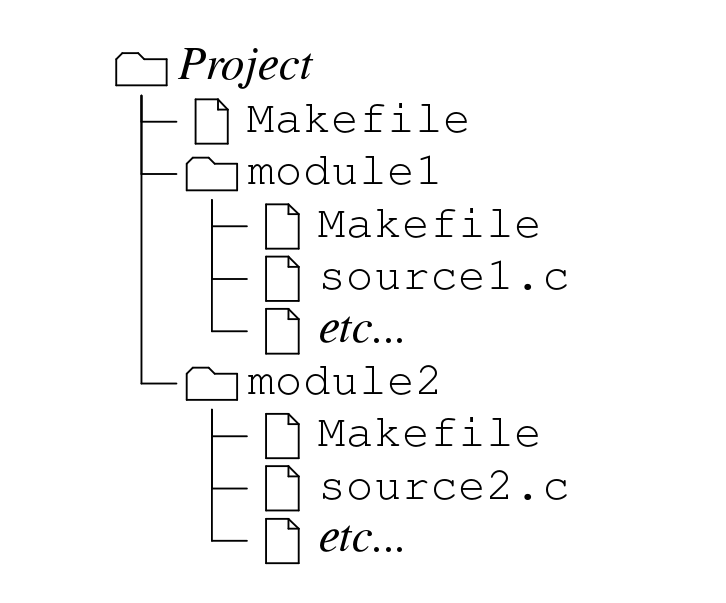
\includegraphics[width=3cm]{structure}
\subsection{Problems}
\begin{enumerate}
\item Difficult to get order of recursion into sub-directories correct - unstable and 
often needs tweaking.
\item Often necessary to do more than one pass over sub-directories - increases build times.
\item Some dependency information is omitted to avoid unreasonable build times.
\item Inter-directory dependencies often omitted or too hard to express, so Makefiles written to 
\textit{over} build to ensure nothing is left out.
\item Inaccurate dependencies lead to the product unable to build cleanly.
\end{enumerate}

\section{What "Make" Does and How It Works}

Give it a set of rules for how to construct things, and a target to be constructed. Rules 
are decomposed into pair-wise ordered dependencies between files. Make takes these files 
and determines how to build the given target. It does this by constructing a
\textit{Directed Acyclic Graph} (DAG).

An example project structure:
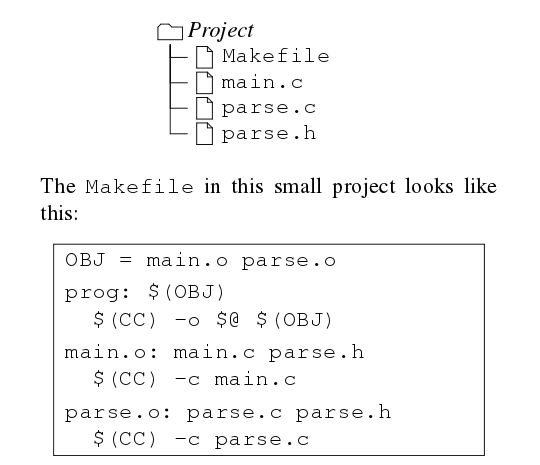
\includegraphics[width=3cm]{simpleproject}

Corresponding Directed Acyclic Graph:
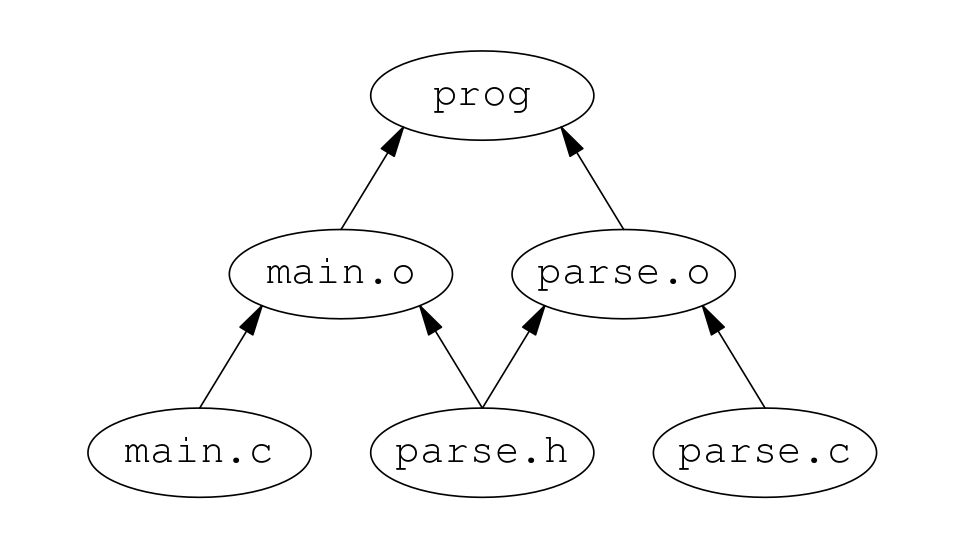
\includegraphics[width=3cm]{dag}

Object files are dependent on the include files \textit{(.h)} even though source files \textit{(.c)} do the including.
This is because if an include file changes, it is the object files that are out-of-date, not the 
source files.

After make has created the DAG, it performs a \textit{postorder} traversal of the DAG. Dependencies are 
visited first. It looks at the last modified of each file, higher files are considered out-of-date if
any of the lower files they depend upon are younger.

Using recursive makes is problematic because it affects both phases: it causes make to construct an
inaccurate DAG, and it forces make to traverse the DAG in an inappropriate order.

Incomplete DAG from recursive make:
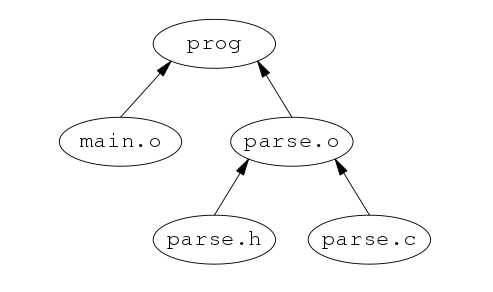
\includegraphics[width=3cm]{incompletedag}

Files are interdependent. Using make recursively means that files created for the next process whilst
unaware of problems such as out-of-date. These out-of-date files are then used as input for later stages
(which \textit{are} aware of being out-of-date), leading to compatibility problems.

\section{Solution}

Use one Makefile for an entire project instead of breaking it up.

\begin{quote}
It is not the recursion itself which is harmful, it is the crippled Makefiles which are used
in the recursion which are wrong.
\end{quote}

It may sound counter-intuitive to have a single Makefile, however the author says that by using \textit{include}
statements, the Makefile is instructed to suspend reading the current one and go to another before continuing.

\section{Conclusion}

This paper is not a typical example of scientific paper, it reads more like a
technical paper. It addresses a real problem related to the misuse of Make to build large projects. The paper 
goes beyond the tutorial like presentations of Make which only state features of the tool and its syntax,
these details can be found in the manuals and
readme files.

Make was designed with the idea that DAG representing the dependency is known beforehand, in such a case 
Make will walk through the dependency graph, recompiling the source files that have been updated and the object 
files that depend on those sources. 

When Makefiles became long and complex the approach proposed to deal with this complexity was to have multiple
makefile distributed over project directory tree breaking the whole idea of Make having a global of view of the
overall dependency of the project. This is turn made the build of large project sometimes unpredictable and 
forces the Makefiles writer either to build too much (multiple traversal of the DAG, or clean the entire project tree)
which does not help to reduce build time of large projects. The rest of the details are only relevant to a person 
who will be facing the problem of creating Manually a makefile for a large software project.	
	\chapter{XML in Atom}

\begin{wrapfigure}{l}{0.5\textwidth}
	\vspace{-10pt}
	\begin{center}
		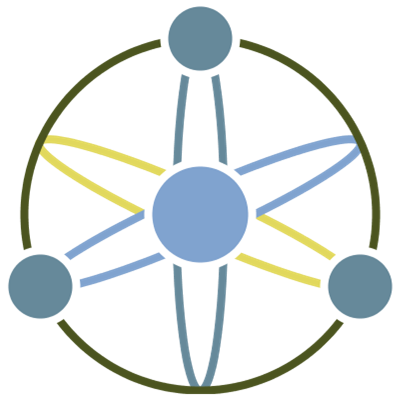
\includegraphics[scale=0.2]{atom-logo.png}
	\end{center}
	\vspace{-10pt}
	\caption{Atom logo.}
	\label{fig:atom_logo}
	\vspace{-10pt}
\end{wrapfigure}

Atom is a web syndication framework and consists of a pair of standards:

\begin{enumerate}
\item Atom Syndication Format - \href{https://tools.ietf.org/html/rfc4287}{RFC 4287}
\item Atom Publishing Protocol - \href{https://tools.ietf.org/html/rfc5023}{RFC 5023}
\end{enumerate}

An Atom feed can consist: plain text, escaped HTML, XHTML, XML, Base64-encoded binary, and references to external content as: documents, video, audio, streams etc.

Unfortunately the official website of the project no longer exists, figure \ref{fig:atom_logo} shows the original Atom project's logo.

\section{Atom Syndication Format}
"Atom is an XML-based document format" (\href{https://tools.ietf.org/html/rfc4287}{RFC 4287, page 3}). The RFC describes how a well-formed Atom document should be formatted.

\section{Atom Publishing Protocol}
This is also known as the "Atom API" and the aim of this project is to improve on and replace the existing XML-RPC-based publishing protocols \cite{xml_com}.

The Atom Publishing Protocol is based on HTTP transfer of Atom-formatted representations, formatted with the Atom Syndication Format \cite{ietf_rfc5023}.

\section{Atom vs. RSS}
Although both the Atom and the RSS standard facilitate the same (a news feed), there are some key differences as shown in table \ref{tab:atomvsrss} below.

\begin{table}[h]
	\begin{tabular}{|l|l|}
	\hline
	Atom & RSS \\ \hline
	Indication of content type & No indication of content type \\
	RFC3339 timestamps & RFC822 timestamps \\
	Supports language ids per readable item & Supports language identifier per article \\
	Reusable elements out of context & Non-reusable elements out of context \\
	\hline
	\end{tabular}
	\caption{Atom vs. RSS}
	\label{tab:atomvsrss}
\end{table}

\section{Atom Document Example}
Atom feeds contain one or more entry sections below the main meta-data section.

\begin{lstlisting}[style=xml, frame=single, caption={feed.xml}]
<?xml version="1.0" encoding="utf-8"?>
<feed xmlns="http://www.w3.org/2005/Atom">

   <title>Example Feed</title>
   <link href="http://example.org/"/>
   <updated>2003-12-13T18:30:02Z</updated>
   <author>
     <name>John Doe</name>
   </author>
   <id>urn:uuid:60a76c80-d399-11d9-b93C-0003939e0af6</id>

   <entry>
     <title>Atom-Powered Robots Run Amok</title>
     <link href="http://example.org/2003/12/13/atom03"/>
     <id>urn:uuid:1225c695-cfb8-4ebb-aaaa-80da344efa6a</id>
     <updated>2003-12-13T18:30:02Z</updated>
     <summary>Some text.</summary>
   </entry>

</feed>
\end{lstlisting}

\subsection{Required feed elements}
The following tags are mandatory when creating an Atom message:
\begin{itemize}
  \item \textbf{id} - Unique and permanent URI identifying the feed
  \item \textbf{title} - Title for the feed
  \item \textbf{updated} - Last time feed was modified
  \item \textbf{author} - At least one, can be more
  \item \textbf{link} - Link to related Web page
\end{itemize}

Optional elements and can be looked found \href{http://www.atomenabled.org/developers/syndication/#optionalEntryElements}{here}. These optionals include details such as initial publication dates and copyright information.

%\end{document}

	\chapter{Group effort}

Group G2, seats 6-11,

\section{Youtube movie Linus Torvalds}
group effort\\
After watching \href{https://www.youtube.com/watch?v=4XpnKHJAok8}{Tech Talk: Linus Torvalds on git} we made some notes.

\subsection{Notes}
balalablabab


\section{Youtube movie unknown}
\textbf{by Jeroen van Prooijen}\\

\begin{wrapfigure}{r}{0.5\textwidth}
 \vspace{-20pt}
 \begin{center}
  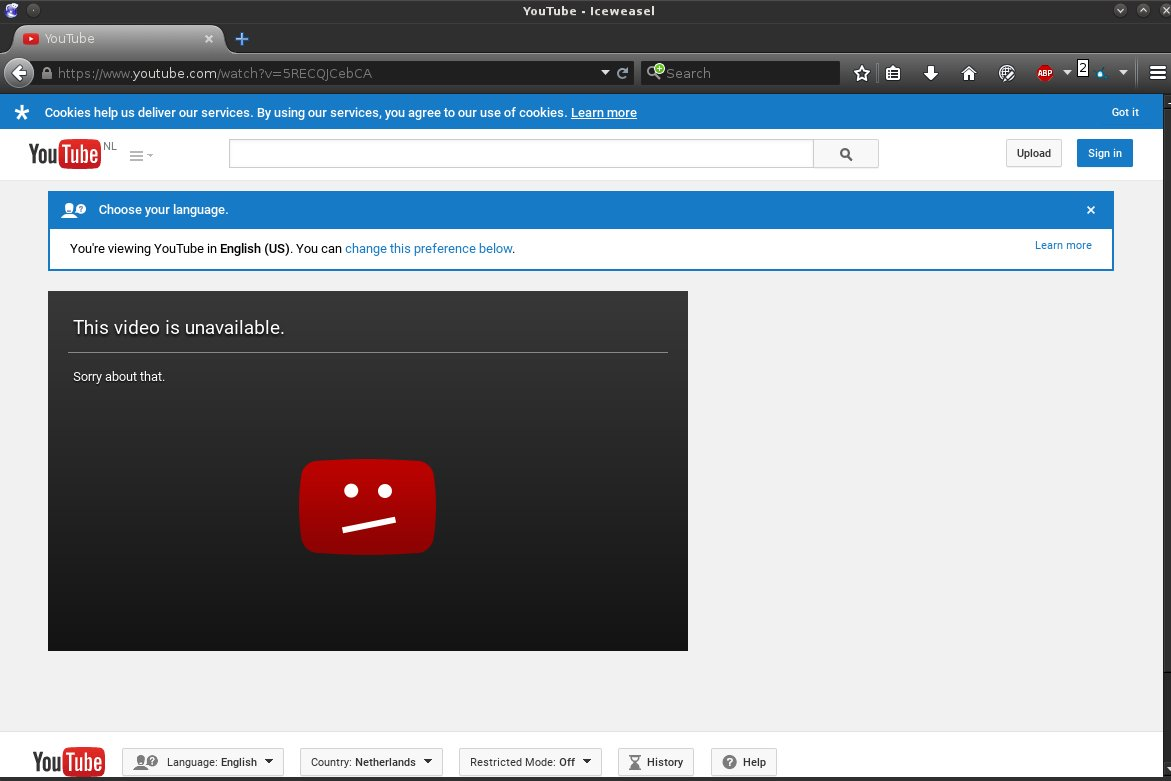
\includegraphics[width=0.5\textwidth]{error_youtube.jpg}
 \end{center}
 \vspace{-20pt}
 \caption{screenshot}
 \vspace{-10pt}
\label{fig:error_youtube}
\end{wrapfigure}

I tried to watch the following youtube movie: \url{https://www.youtube.com/watch?v=5RECQJCebCA}\\
but it could not be found, see image \ref{fig:error_youtube}. For the placing the image \ref{fig:error_youtube} and wrapping this
text around it I used a explanation on Wikibooks.org\cite{wikibooks_figures}

\newpage

\section{LaTeX vs Word}
\textbf{by Mike Maarse}\\

\section{Stackexchange links}
\textbf{by Tom Curran}\\


	\bibliographystyle{plain}	
	\bibliography{biblio}
	\listoffigures
\end{document}